\section{John Nash and the Complexity of Solving Integration: Why It's Like Cracking Encryption (1955)}

\subsection{John Nash and the Complexity of Computation}

In the post-war mathematical renaissance of the mid-20th century, a young prodigy named \textbf{John Nash} arrived at Princeton with a one-sentence letter of recommendation:  ``This man is a genius.''

He was. By age 21, Nash had revolutionized \textbf{game theory} with what would become the \textit{Nash Equilibrium}—a concept that formalized strategic stability in games involving multiple decision-makers. But while Nash is most famous for this breakthrough, the deeper implications of his work were only just beginning to surface.

In his 1950–51 papers, Nash proved the existence of equilibrium in finite games using \textbf{fixed-point theorems} (notably Brouwer’s). These theorems are \textit{non-constructive}—they guarantee a solution exists, but provide no method for actually finding it. This opened a mathematical Pandora’s box:

\begin{itemize}
    \item How hard is it to compute a Nash equilibrium?
    \item Can we find one efficiently—in polynomial time?
    \item Is the problem harder in multiplayer games than in two-player ones?
\end{itemize}

These questions wouldn’t be formalized until decades later, but they retroactively placed Nash’s equilibrium in the center of \textbf{computational complexity theory}. It became the prototype of a problem that is mathematically guaranteed to exist, but potentially \textit{intractable}. 

And Nash saw it coming. Even before the rise of P vs.\ NP, he was already thinking about the hardness of solving problems—not just in terms of mathematical structure, but in terms of \textbf{computational effort}.

This foresight became most evident in his cryptographic work during the Cold War. In a now-declassified letter to the NSA, Nash warned that any cryptographic system which could be broken by a machine using only a ``relatively small number of operations'' should be considered insecure. In other words: if you can compute the answer too quickly, the system is broken. The problem must be \textit{computationally hard}.

In this light, Nash’s contributions go far beyond equilibrium theory. He helped define a new kind of difficulty—\textbf{computational difficulty}—and sketched the outlines of complexity theory before the field even had a name.

\subsection{Cryptography and Exponential Time}

In the early 1950s, Nash was involved in \textbf{classified cryptographic work} for the U.S. government during the Cold War. He proposed a number of encryption schemes and ideas to the National Security Agency (NSA), including a one-way function system that remarkably resembled concepts later formalized in \textit{public-key cryptography}.

In one now-declassified letter to the NSA from 1955, Nash warned that cryptographic systems must be designed with extreme care because adversaries could apply massive computational brute-force attacks. He explicitly stated:

\begin{quote}
``I hope my work in this field may seem worthwhile… but I must caution that any cryptographic method which can be broken by a computing machine using only a relatively small number of operations... should be considered insecure.''
\end{quote}

Here, Nash hit upon a key insight: \textbf{the strength of a cryptographic system depends on its resistance to fast, general-purpose algorithms}. His comment prefigured the field of \textit{complexity theory}, and especially the study of problems for which no known efficient (polynomial-time) solution exists.

These were not abstract concerns. The NSA was locked in a mathematical arms race with Soviet code-breakers, and Nash's suggestions were meant to address real-world vulnerabilities. In that environment, Nash recognized that the \textit{hardness} of certain problems—those involving vast combinatorial spaces or deep symmetries—wasn’t just a computational inconvenience. It was a strategic weapon.

\begin{tcolorbox}[title=Historical Sidebar: John Nash and the Logic of Delusion, colback=gray!5, colframe=black, fonttitle=\bfseries]

  John Nash is best known for his revolutionary work in mathematics and economics—most famously, his development of the \textbf{Nash equilibrium}, which redefined modern game theory. But alongside the elegant logic of strategic decision-making, Nash lived through something far less rational: a prolonged descent into \textbf{paranoid schizophrenia}.

  \medskip
  
  Beginning in the late 1950s, Nash began to exhibit signs of psychosis. He believed foreign governments were communicating with him through coded messages. He saw conspiracies everywhere. At one point, he claimed he was a political figure with a secret mission, at another, that extraterrestrials were directing his life. 

  \medskip
  
  But what made Nash’s illness so unsettling was that his delusions were not incoherent. In fact, they were disturbingly logical—\textbf{structured systems built on faulty premises}. The same mind that could formalize game theory was now formalizing hallucinations. He wasn’t seeing chaos; he was constructing alternate realities that made perfect internal sense.
  
  \medskip
  
  Years later, Nash described his recovery as an intellectual act—not the disappearance of hallucinations, but the slow, rational rejection of their premises:

  \medskip
  
  \ 

  \begin{quote}
      \textit{"I began to intellectually reject some of the delusionally influenced lines of thinking... and eventually I intellectually established a growing ability to discard them."}
  \end{quote}
  
  \medskip
  
  The moral is as profound as it is unsettling: \textbf{reason alone is not self-validating}. Logic is only as sound as the assumptions it rests on. Even a flawless line of reasoning can lead to madness if it starts from the wrong place. 
  
  \medskip
  
  Nash was a genius, but his story is a warning: \textbf{without a proper foundation, even reason can become a prison.}
  
\end{tcolorbox}



\subsection{Exponential Growth and Intractability}

Nash speculated that many problems, particularly those involving encryption, optimization, or prediction under uncertainty, might require \textbf{exponential time} to solve. That is: the time it takes to find a solution could grow explosively with the size of the problem, quickly outpacing any feasible computational resources.

This intuition foreshadowed what computer scientists would later formalize as the distinction between \textbf{tractable (P)} and \textbf{intractable (NP-hard)} problems. Nash didn’t have the modern vocabulary, but he had the vision.

To illustrate this, consider a classic example: the \textit{Traveling Salesman Problem}. Find the shortest route that visits each city exactly once and returns to the start. With just a few cities, the task is easy. With 20? Millions of possibilities. With 50? Practically unsolvable by brute force. This kind of \textbf{combinatorial explosion} is exactly the sort of difficulty Nash gestured toward.

\medskip

In retrospect, Nash’s early remarks on computational hardness—made in the context of encryption and national security—were startlingly prescient. They show that even in a time before complexity theory had a name, its shadow had already fallen across the minds of the greatest mathematicians. Nash saw what many would only later articulate: some problems are not just difficult—they are \textbf{structurally resistant} to being solved efficiently.


\subsection{Implications for Modern Problems}

When we think about tasks like training deep learning models, it’s easy to see how the problem scales. These models learn by optimizing—adjusting their internal parameters to better fit the data. The complexity grows as the model becomes larger and the data set expands. The analogy to Nash’s speculation holds: solving the optimization problem with millions of parameters or vast amounts of data can take an exponential amount of time, especially when exact solutions are required.

This means that the methods we use to tackle these problems often need to be very creative. In many cases, brute force (trying every possible solution) simply doesn’t work. Instead, we rely on approximations, simplifications, or heuristics to make the problem solvable in a reasonable amount of time.

\subsection{The Role of Insight in Solving Hard Problems}

Despite the computational challenges, there is always a way to make problems more manageable by using insights. Just as Nash’s work showed that game theory could simplify decision-making in competitive situations, we can also apply insight to simplify computational problems. For instance, finding patterns, leveraging symmetries, or transforming the problem into a different form can reduce the complexity and make what once seemed impossible a lot more manageable.

In computational tasks like optimization, the trick is often not just to throw more computational resources at the problem, but to reframe the problem in a way that makes it easier to solve. This kind of cleverness is what separates practical solutions from intractable ones.

While some problems will always require significant computational effort, the key to tackling these challenges lies in understanding when computation will become impractical and when insight can simplify the problem. As Nash’s speculations highlight, not every problem is solvable quickly, and knowing when to apply cleverness and creativity is as important as knowing when to apply raw computational power.

In the next sections, we’ll look at how this interplay between creativity, insight, and computational difficulty applies to problems like solving the wave equation and simulating physical systems, such as gravity and orbital mechanics. We’ll explore how mathematical solutions evolve over time and how computational complexity affects the strategies we choose to solve real-world problems.

\subsection{The Puzzle: One Heavy Marble Among Many}

Imagine a bag with 128 marbles. One of them is slightly heavier than the others, but all the rest are identical in weight. You have no idea which one it is, and you can’t feel the difference by hand. However, you do have access to a balance scale—one of those old-fashioned devices that lets you compare the weights of two groups of objects. Your goal is simple: find the heavy marble using as few comparisons as possible.

This might sound like a fun parlor game, but it’s actually a beautiful analogy for computational complexity. Each strategy you use to solve the problem can be thought of as an algorithm. And the number of weighings required reflects the time complexity of that algorithm.

Let’s look at three strategies, each illustrating deeper insight into reducing computational effort.

\subsubsection{Strategy 1: Brute Force Weighing}

The most direct approach is to weigh each marble individually. Take one marble out, place it on one side of the balance, and compare it to each of the other marbles one by one. Eventually, the heavier marble will tip the scale.

As a motivating example, suppose we have 128 marbles. In the worst-case scenario, the heavy marble might be the last one we test—after 127 comparisons. This isn't just slow, it’s inefficient.

\textbf{More generally:} for any \( n \) marbles, brute force takes at most \( n - 1 \) weighings in the worst case. This is an example of a \textbf{linear-time algorithm}, written in Big-O notation as \( O(n) \). That means the time required to solve the problem grows proportionally with the number of marbles.

\medskip

\noindent\textbf{Qualitative Insight:} Imagine lining up all the marbles and testing them one by one. Each test adds one more unit of time. As the number of marbles increases, so does the total effort. If you double the number of marbles, you double the number of weighings. If you triple it, you triple the time. This is what defines a linear relationship between problem size and time.

\begin{center}
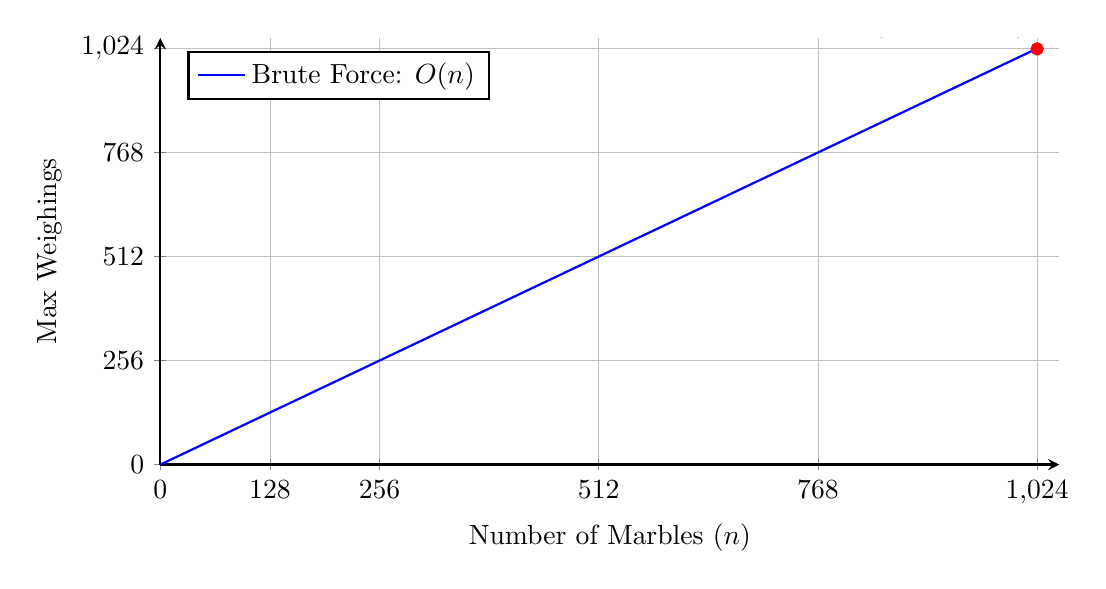
\begin{tikzpicture}
  \begin{axis}[
    width=13cm,
    height=7cm,
    grid=both,
    grid style={line width=.1pt, draw=gray!10},
    major grid style={line width=.2pt,draw=gray!50},
    axis lines=left,
    xlabel={Number of Marbles (\(n\))},
    ylabel={Max Weighings},
    ymin=0, ymax=1050,
    xmin=0, xmax=1050,
    xtick={0, 128, 256, 512, 768, 1024},
    ytick={0, 256, 512, 768, 1024},
    domain=0:1024,
    samples=100,
    smooth,
    thick,
    legend style={at={(0.03,0.97)}, anchor=north west}
  ]
    \addplot [blue] {x};
    \addlegendentry{Brute Force: \( O(n) \)}
    
    % Highlight point at n = 1024
    \addplot[only marks, mark=*, mark size=2pt, red] coordinates {(1024,1023)};
    \node[anchor=south east, red] at (axis cs:1024,1023) {$(1024,\ 1023)$};

  \end{axis}
\end{tikzpicture}
\end{center}



\noindent In the graph above, you can see the linear relationship: as the number of marbles increases, the number of weighings rises at the same rate. The red point marks our motivating example: 128 marbles requiring up to 127 comparisons.

This strategy is easy to implement and requires no cleverness—but the cost of that simplicity is speed. As we'll see in the next strategies, smarter approaches can achieve dramatically better scaling by reducing the number of comparisons needed.


\subsubsection{Strategy 2: Divide and Conquer}

A much more efficient approach is to use a \textbf{binary search strategy}. Instead of checking marbles one at a time, you divide them into two equal groups and weigh those groups against each other.

\medskip

\noindent\textbf{Example:} With 128 marbles, split them into two groups of 64 marbles. Weigh them:
\begin{itemize}
  \item If one side is heavier, the heavy marble is in that group.
  \item If the weights are equal, this (in a more general version of the problem) would help—but here, since we know one is heavier, the heavier side always contains the odd one out.
\end{itemize}

You now repeat the process, halving the number of marbles at each step: 64, 32, 16, 8, 4, 2, and finally 1.

\[
\log_2(128) = 7
\]

So in just \textbf{7 weighings}, you can guarantee you’ll find the heavy marble.

\medskip

\noindent\textbf{General Case:} For any \( n \), this strategy takes at most \( \log_2(n) \) steps. This is a \textbf{logarithmic-time algorithm}, or \( O(\log n) \). As \( n \) increases, the number of steps grows very slowly in comparison.

\medskip

\noindent\textbf{Qualitative Insight:} Halving the problem size at every step is incredibly powerful. Instead of scaling linearly with the number of items, the number of steps increases much more slowly. If you double the number of marbles, you only add one more weighing. This makes binary search a cornerstone of efficient algorithms.

\begin{center}
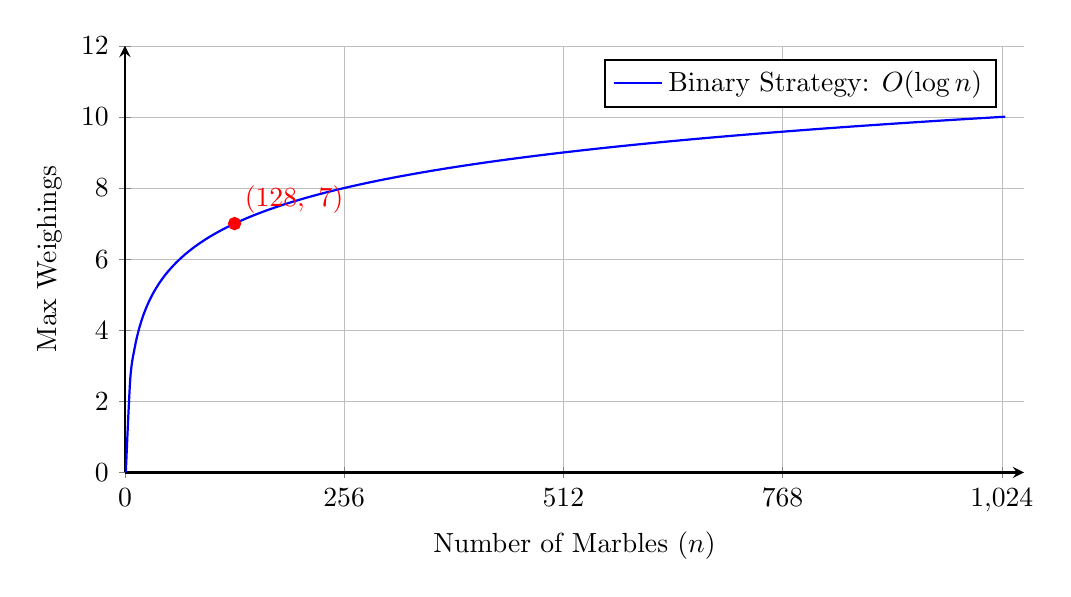
\begin{tikzpicture}
  \begin{axis}[
    width=13cm,
    height=7cm,
    grid=both,
    grid style={line width=.1pt, draw=gray!10},
    major grid style={line width=.2pt, draw=gray!50},
    axis lines=left,
    xlabel={Number of Marbles (\(n\))},
    ylabel={Max Weighings},
    ymin=0, ymax=12,
    xmin=0, xmax=1050,
    xtick={0, 256, 512, 768, 1024},
    ytick={0,2,4,6,8,10,12},
    domain=1:1028,
    samples=200,
    smooth,
    thick,
    legend style={at={(0.97,0.97)}, anchor=north east}
  ]
    % Logarithmic curve
    \addplot [blue] {log2(x)};
    \addlegendentry{Binary Strategy: \( O(\log n) \)}

    % Highlight point at 128 marbles
    \addplot[only marks, mark=*, mark size=2pt, red] coordinates {(128,7)};
    \node[anchor=south west, red] at (axis cs:128,7) {$(128,\ 7)$};
  \end{axis}
\end{tikzpicture}
\end{center}

\noindent The chart above shows the number of weighings needed for various \( n \) using the binary strategy. The growth curve rises quickly at first but then flattens. Even for large \( n \), the number of weighings remains manageable. The red point marks the 128-marble example: 7 steps to find the heavy one.

\medskip

This strategy reflects the power of \textbf{divide and conquer}—breaking a large problem into smaller subproblems, solving them independently, and combining the results. It’s a key design pattern in efficient algorithms, and a big reason why many large-scale problems are solvable in practice.

\subsubsection{Strategy 3: Ternary Elimination (Base-3 Strategy)}

It gets even better. What if, instead of dividing the marbles into two groups, we divide them into \textbf{three}?

\begin{itemize}
  \item Group A: 42 marbles
  \item Group B: 42 marbles
  \item Group C: 44 marbles
\end{itemize}

We weigh Group A against Group B:
\begin{itemize}
  \item If the weights are equal, the heavy marble must be in Group C.
  \item If one side is heavier (say Group A), then the heavy marble is in that group, and the other two groups can be eliminated.
\end{itemize}

Each weighing in this strategy reduces the search space to one-third its previous size—an even more aggressive cut than halving. In computational terms, this gives us a time complexity of:
\[
\log_3(n)
\]

\medskip

\noindent\textbf{Example:} For \( n = 128 \), we have:
\[
\log_3(128) \approx 4.76
\]
So in the worst case, we only need \textbf{5 weighings}. That’s even better than the 7 steps required by binary search.

\medskip

\noindent\textbf{Qualitative Insight:} Imagine shrinking your search space by two-thirds at each step. That’s an enormous speedup. As the number of marbles grows, the number of steps increases—but incredibly slowly. Even for 1,000 marbles, you’d still need fewer than 7 comparisons.

This is a \textbf{base-3 search}, and it’s \textbf{provably optimal} for balance-scale comparisons. No algorithm can beat it using a standard scale with three outcomes: heavier left, heavier right, or equal.

\begin{center}
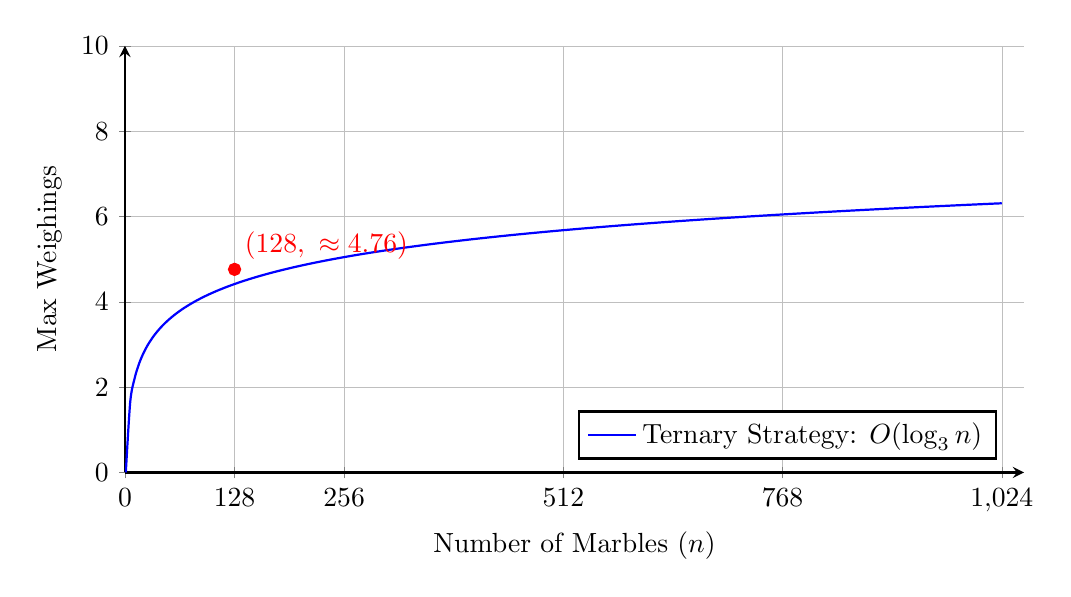
\begin{tikzpicture}
  \begin{axis}[
    width=13cm,
    height=7cm,
    grid=both,
    grid style={line width=.1pt, draw=gray!10},
    major grid style={line width=.2pt, draw=gray!50},
    axis lines=left,
    xlabel={Number of Marbles (\(n\))},
    ylabel={Max Weighings},
    ymin=0, ymax=10,
    xmin=0, xmax=1050,
    xtick={0, 128, 256, 512, 768, 1024},
    ytick={0,2,4,6,8,10},
    domain=1:1024,
    samples=200,
    smooth,
    thick,
    legend style={at={(0.97,0.03)}, anchor=south east}
  ]
    % Use ln(x)/ln(3) for base-3 log
    \addplot [blue] {ln(x)/ln(3)};
    \addlegendentry{Ternary Strategy: \( O(\log_3 n) \)}

    % Manually insert the highlight point
    \addplot[only marks, mark=*, mark size=2pt, red] coordinates {(128, 4.76)};
    \node[anchor=south west, red] at (axis cs:128,4.76) {$(128,\ \approx 4.76)$};
  \end{axis}
\end{tikzpicture}
\end{center}



\noindent The graph above shows how slowly the number of weighings increases with the number of marbles using the ternary elimination method. For 1024 marbles, the maximum number of weighings is:
\[
\log_3(1024) \approx 6.3
\]
—still only \textbf{7 steps in the worst case}!

\medskip

This is why ternary search isn’t just clever—it’s \textbf{as good as it gets}. It demonstrates how understanding the structure of your problem can lead to exponential speedups.

\subsubsection{Why We Can't Do Better: The Information-Theoretic Limit}

You might wonder: is there a strategy even better than dividing into three groups? Could we somehow guess the heavy marble in fewer than \( \log_3(n) \) steps?

To answer that, we turn to a fundamental concept from information theory: \textbf{entropy}, which you can think of as a way of measuring uncertainty. The more uncertainty we have, the more information we need to resolve it.

Imagine this: you have 128 marbles in a bag, and you know exactly one of them is heavier than the rest. But you don’t know which one. From your perspective, any of those 128 marbles could be the special one—they’re all equally likely. That’s a lot of uncertainty.

Now here’s the key idea: \textit{to identify the heavy marble, we need to ask enough yes/no questions to rule out all the others}. Think of it like a game of 20 Questions—but where each question can only be answered with a “yes” or “no,” and every answer helps you narrow down the options.

Each yes/no question gives you one “bit” of information—a binary choice. After one bit, you’ve split the group into 2. After two bits, you’re down to 4 groups. After three bits, 8 groups. And so on. The number of possibilities shrinks exponentially with each bit of information you gain.

So how many bits do you need to shrink 128 possibilities down to just one? That’s what \( \log_2(128) \) tells you: the number of times you have to divide the space in half to get down to a single possibility. In this case, \( \log_2(128) = 7 \). That means we need \textbf{7 bits of information}—or, equivalently, \textbf{7 carefully chosen yes/no questions}—to find the heavy marble.

Entropy is just a formal way of quantifying this: \textit{how many bits of information are needed to resolve uncertainty in a system with many possible outcomes?}


\begin{center}
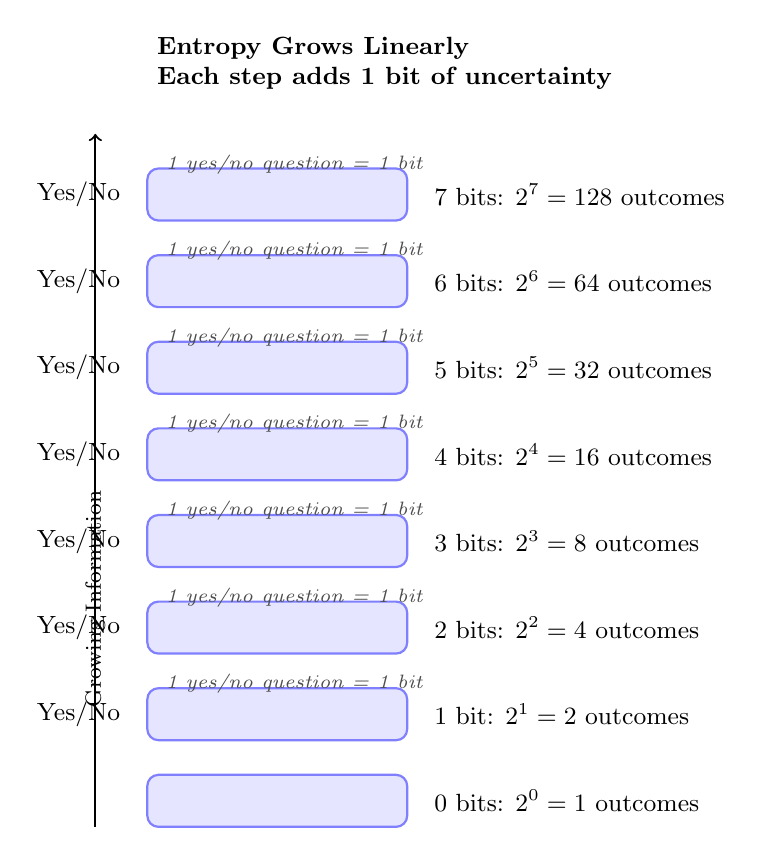
\begin{tikzpicture}[
  yscale=1.1,
  xscale=1.1,
  every node/.style={font=\small}
]

% Draw horizontal bars for each bit layer
\foreach \y/\bits/\outcomes in {
  0/0/1,
  1/1/2,
  2/2/4,
  3/3/8,
  4/4/16,
  5/5/32,
  6/6/64,
  7/7/128
} {
  % Bar
  \draw[fill=blue!10, draw=blue!50, thick, rounded corners] (0,\y) rectangle (3,\y+0.6);
  
  % Entropy label
  \node[anchor=west] at (3.2, \y+0.3) {\(\bits\) bit\ifnum\bits=1\else s\fi: \(2^{\bits} = \outcomes\) outcomes};
  
  % Yes/No label (skip bit 0 for simplicity)
  \ifnum\bits>0
    \node[anchor=east] at (-0.2, \y+0.3) {Yes/No};
    \node[anchor=west, font=\scriptsize\itshape, gray!60!black] at (0.1, \y+0.65) {1 yes/no question = 1 bit};
  \fi
}

% Label on top
\node[align=left, anchor=south west, font=\small\bfseries] at (0, 8.4) {
  \textbf{Entropy Grows Linearly} \\
  Each step adds 1 bit of uncertainty
};

% Arrow showing upward growth
\draw[->, thick] (-0.6, 0) -- (-0.6, 8) node[midway, left, rotate=90, font=\footnotesize] {Growing Information};

\end{tikzpicture}
\end{center}






Now let’s think about what we actually get from each weighing. A balance scale doesn’t just say “yes” or “no” — it gives us one of three outcomes: the left side is heavier, the right side is heavier, or the two sides are perfectly balanced. That means each weighing doesn’t just split the possibilities in half — it splits them into three parts.

From an information perspective, that’s powerful: instead of just asking a yes/no question (which gives us 1 bit of information), each weighing gives us a little more — about \( \log_2(3) \approx 1.584 \) bits of information. It’s like squeezing more juice out of every question.

But remember, we still have the same total uncertainty to resolve — \( \log_2(n) \) bits if we’re trying to find one special item out of \( n \). So the question becomes: how many weighings do we need if each weighing gives us only 1.584 bits?

The answer is: take the total amount of uncertainty, and divide it by how much each weighing tells you. That gives us:
\[
\frac{\log_2(n)}{\log_2(3)} = \log_3(n)
\]

So even though the scale gives us more than 1 bit per question, we still need multiple weighings to gather enough information to uniquely identify the heavy marble. And now we know exactly how many: at least \( \log_3(n) \) weighings.


In our case, we’re working with 128 marbles. That means we need to gather enough information to narrow down from 128 possibilities to just one. And since each weighing gives us about 1.584 bits of information, we can ask: how many weighings would it take to get at least 7 bits?

The answer is:
\[
\log_3(128) \approx 4.76
\]
In other words, even in the best-case scenario, we need at least 5 weighings to identify the heavy marble. And as we’ve seen, there’s a clever strategy that does exactly that — so we’re already doing as well as we possibly can.

This isn’t just a coincidence or a clever trick. It’s a mathematical limit. Think of every weighing as a question with three possible answers. If you draw out all the possible sequences of answers — left heavier, right heavier, or equal — you get a tree where each step branches three ways. To cover all 128 marbles, that tree needs at least 128 leaves.

And the only way to fit that many leaves is to make the tree at least 5 levels deep. That’s the minimum number of weighings needed to guarantee you can tell every marble apart. No matter how clever the strategy, you can’t shrink the problem any further without breaking the rules.

So the base-3 elimination method isn’t just efficient — it’s \textit{provably optimal}. It’s the best possible strategy given the rules of the game.





\subsubsection{Why This Matters: Algorithms, Complexity, and Insight}

This marble game is more than a clever puzzle—it models how we think about computational efficiency. Each weighing is like a computational step. Brute-force methods take too long for large problems. Divide-and-conquer strategies are better. And the most insightful approaches—like the ternary strategy—reframe the problem entirely and exploit the structure to reduce effort.

Just as Nash hinted, some problems grow exponentially harder as they scale. But with the right insight, we can cut through that complexity. Understanding the limits of what’s possible—like proving that no strategy can beat \( \log_3(n) \) comparisons—is at the heart of computational theory.

In the next section, we’ll see how similar principles apply to solving equations in physics, simulating gravity, and understanding how nature itself may ``compute'' the evolution of systems—sometimes efficiently, sometimes not.



\subsection{Bounding Problems with Big-O Notation}

Now that we’ve explored different strategies for solving the heavy marble puzzle, we can take a step back and talk more generally about a key idea in computational theory: \textbf{bounding how hard a problem is}.

In computer science, we use something called \textbf{Big-O notation} to describe how the time (or steps) needed to solve a problem grows as the size of the input increases. It’s a way of saying, “Even if we don’t know the exact number of operations, we know the \emph{trend}.”

\medskip

\noindent\textbf{Back to marbles:} In the brute-force strategy, we saw that checking each marble individually takes at most \( n - 1 \) comparisons. We write this as:
\[
O(n)
\]
That’s linear time. The time it takes grows directly with the number of marbles.

With binary search, we showed that the number of weighings grows like \( \log_2(n) \). So we write:
\[
O(\log n)
\]
And with the ternary strategy, we tightened that even further. Since we \textit{proved} you can’t do better than \( \log_3(n) \) weighings — and we have a strategy that achieves that — we say this problem has a \textbf{logarithmic lower bound}. The problem is \textit{bounded} by:
\[
O(\log n)
\]
We can say this with confidence because the information-theoretic argument showed that no matter how clever the strategy, we can't beat that limit.

\medskip

\noindent\textbf{Why this matters:} Not every problem is so cooperative. In fact, many problems don’t scale as nicely. Some grow:
\begin{itemize}
  \item In polynomial time: \( O(n^2),\ O(n^3), \) etc.
  \item In exponential time: \( O(2^n) \)
  \item In factorial time: \( O(n!) \)
\end{itemize}

These aren’t just abstract labels — they tell us something very real about whether a problem can be solved efficiently. If a problem takes exponential time, that means the number of steps doubles with every extra input unit. That quickly becomes impossible for any computer to handle. A problem that takes \( O(n!) \) time? Even worse — you’re dead before it finishes.

\medskip

\noindent\textbf{So what’s the goal?} To understand which problems fall into which classes. Some problems have clever algorithms that make them tractable. Others have no known efficient solution, and might not have one at all. And in the most challenging cases, we can even \textit{prove} that no efficient algorithm can ever exist — that a problem is fundamentally hard, no matter how much hardware or cleverness we throw at it.

\medskip

We’ll explore those classes — like \textbf{P}, \textbf{NP}, and \textbf{NP-complete} — in upcoming sections. But it all begins here, with the idea that problems have intrinsic complexity, and that Big-O notation helps us describe their boundaries.




\subsection{Computational Complexity: Solving vs.\ Verifying}

So far, we've explored entropy, search strategies, and the power of asking the right questions. But there's a deeper question lurking underneath all of this: \emph{Is it easier to check an answer than to find it?}

This question sits at the heart of computational complexity theory—and leads to one of the most important distinctions in computer science: the difference between \textbf{solving} a problem and \textbf{verifying} a proposed solution.

\medskip

\noindent Suppose someone hands you an answer to a complex problem. Can you quickly tell if it's correct? If so, we say the problem is \textbf{verifiable in polynomial time}. This defines the class:

\begin{itemize}
  \item \textbf{NP} (nondeterministic polynomial time): problems for which a solution, once given, can be checked efficiently.
\end{itemize}

But not all problems in NP are easy to solve. That's where \textbf{P} comes in:

\begin{itemize}
  \item \textbf{P}: Problems that can be both solved and verified in polynomial time. These are the ones we love—clean, efficient, and scalable.
\end{itemize}

The real drama happens in the space between P and NP:

\begin{itemize}
  \item \textbf{NP-Complete}: These are the hardest problems in NP. They can be verified quickly but aren’t known to be solvable quickly. Crucially, if you could solve one of them efficiently, you could solve all of NP efficiently. They represent the tipping point: the “hardest of the easy-to-check.”
  \item \textbf{NP-Hard}: These problems are at least as hard as NP-complete problems, but they’re \emph{not necessarily in NP}—which means they may not even have efficiently checkable solutions. You can’t even verify the answer in polynomial time, let alone find it.
\end{itemize}

Now let’s scale up.

\begin{itemize}
  \item \textbf{EXP}: Problems solvable in exponential time. These are technically solvable, but only if you have time measured in cosmic epochs.
  \item \textbf{NEXP}: This is the verification analog of EXP. These are problems whose solutions can be verified by a nondeterministic machine in exponential time. In the same way that NP is the “verifiable version” of P, NEXP is the “verifiable version” of EXP.
\end{itemize}

\medskip

\noindent In summary, complexity classes tell us:

\begin{itemize}
  \item Which problems are solvable quickly (P)
  \item Which problems are only checkable quickly (NP)
  \item Which problems aren’t even checkable in reasonable time (NP-Hard and beyond)
  \item And how solvability and verifiability diverge as problems scale from polynomial to exponential time (P → NP and EXP → NEXP)
\end{itemize}

\noindent These distinctions aren’t just theoretical—they determine what kinds of problems we can automate, what we can prove, and what we’ll spend decades approximating.

In the next sections, we’ll explore how integration and related symbolic computation problems land in this complexity landscape—and why they often push us beyond P and into the realm of exponential or even undecidable territory.




\subsection{A Guided Tour Through Computational Complexity}

Computational complexity is the art of classifying problems by how hard they are to solve or verify. Some problems are easy. Some are manageable. Some are mind-bendingly hard. And some are so difficult that even a universe-sized computer wouldn't help.

This section introduces major complexity classes with a single recurring analogy: you're given a list of numbers and asked to solve a number puzzle. The nature of the puzzle changes depending on the class.

\subsubsection{P: Problems Solvable in Polynomial Time}

\textbf{Analogy: Is the number 42 in the list?} \\
You can check each number one by one, and you'll finish in reasonable time even for big lists. These problems are considered "tractable": solvable efficiently as their input grows.

\textbf{Formal definition:} P is the class of decision problems solvable by a deterministic Turing machine in polynomial time.

Life is good in P. These are the problems we can actually solve in practice.

\subsubsection{NP: Problems Verifiable in Polynomial Time}

\textbf{Analogy: Do any three numbers in the list sum to 42?} \\
You can't easily find the right triplet — but if someone shows you three numbers, you can quickly verify whether they work.

\textbf{Formal definition:} NP is the class of decision problems solvable in polynomial time by a non-deterministic Turing machine, or equivalently, problems for which a solution can be verified in polynomial time.

Many real-world problems fall here — scheduling, puzzles, pathfinding — even if finding the solution is tough, we can check it fast.

\subsubsection{NP-Complete: The Hardest of the Easy-to-Check Problems}

\textbf{Analogy: Among all problems where a solution can be verified quickly, this is the most devious version of "Do three numbers sum to 42?"} \\
NP-Complete problems are the toughest members of NP. If you solve one of them quickly, you could solve \emph{all} NP problems quickly.

\textbf{Examples:} SAT, 3SAT, Subset Sum, Hamiltonian Path

\textbf{Why it matters:} NP-complete problems represent the boundary between hard problems we can check, and the unknown world of whether we can actually solve them quickly.

\subsubsection{NP-Hard: So Hard, Even Guessing Doesn’t Help}

\textbf{Analogy: Optimize 3 conflicting diet constraints, maximize taste, and minimize cost — with unknown ingredients} \\
These problems are at least as hard as the hardest NP problems, but they may not be in NP themselves (i.e., their solutions may not even be verifiable in polynomial time).

\textbf{Examples:} TSP with weights, general optimization problems, halting problem (undecidable but NP-Hard)

\textbf{Note:} NP-Complete $\subset$ NP-Hard, but NP-Hard also includes problems outside of NP.

\subsubsection{EXP: Problems Solvable in Exponential Time}

\textbf{Analogy: Evaluate every possible move in a giant game of chess on an $n \times n$ board} \\
You can solve it — but only by checking an exponential number of configurations. These problems live in a class where solving time grows like $2^n$, $3^n$, or worse.

\textbf{Formal definition:} EXP is the class of problems solvable by a deterministic Turing machine in exponential time.

\textbf{Examples:} Generalized Chess, Go, or checking the winner of a massive logical game. Problems that require exploring a full exponential space.

\subsubsection{NEXP: Non-Deterministic Exponential Time}

\textbf{Analogy: You're allowed to guess a cosmic-sized chess move and verify it using galactic resources} \\
This is the non-deterministic version of EXP — you can "magically guess" a solution and verify it in exponential time.

\textbf{Examples:} Quantified Boolean Formulas (QBF), certain verification tasks in logic and formal methods.

\textbf{Significance:} NEXP contains problems whose verification requires exponential effort — like checking every possible strategy in a multiverse of moves.

\subsubsection{A Sidebar on Integration}

Symbolic integration, surprisingly, lives somewhere between NP-Hard and EXP. Finding a closed-form integral requires searching a symbolic space that may grow super-polynomially. While verifying a candidate (by differentiation) is easy, finding one is often deeply non-trivial — sometimes impossible in elementary terms. The Risch Algorithm handles this but can behave like an exponential-time beast.

\textbf{Analogy:} You're asked to find a formula for a secret recipe (an antiderivative), but the kitchen is infinite, and the ingredients include transcendental functions and nested radicals.

\vspace{1em}
This landscape gives us a map — from the efficiently solvable to the incomprehensibly complex. And while P vs. NP remains unsolved, what’s clear is that some problems are harder not just in degree, but in kind.


\subsection{Differentiation is P; Integration is NP-Hard}

So where does \textbf{integration} fall in this spectrum?

\textit{Somewhere between NP-Hard and EXP.}

Why? Because integration is inherently non-local. It doesn’t just care about what’s happening at a single point like differentiation does—it cares about the entire function’s behavior.


In the world of computational complexity:

\begin{itemize}
  \item Differentiation is like class \textbf{P}. It’s efficient, local, and rule-following. You apply the chain rule, product rule, and off you go.
  \item Integration is like \textbf{NP-hard}. It requires knowing the entire structure of the function. You might need substitutions, clever identities, or transformations pulled from the depths of mathematical lore.
\end{itemize}

This is why most integrals you meet in real-world physics can’t be solved exactly. There’s no universal “integration formula” because integration is fundamentally non-local—it demands a global understanding of the function.

\subsection{Why We Need Numerical Integration}

Because exact solutions are often impossible, we rely on approximations:

\begin{itemize}
  \item \textbf{Trapezoidal rule}: slice the area under the curve into trapezoids.
  \item \textbf{Simpson’s rule}: fit parabolas between points.
  \item \textbf{Monte Carlo methods}: estimate integrals with random sampling.
\end{itemize}

These are the numerical hammers we use when the analytical nails won’t budge. They’re essential tools—but they don’t give insight. They give numbers.

\subsection{Orbital Mechanics: When Integration Bites Back}

We’ve argued that integration isn’t just mathematically challenging—it’s computationally brutal. Now let’s look at a real-world example where this difficulty becomes inescapably clear: simulating gravitational systems.

\subsubsection{Why We Can’t Just “Solve” Gravity}

Consider Newton’s law of gravity in its rawest, most unforgiving form:

\[
\frac{d^2\vec{r}}{dt^2} = -\frac{GM}{r^2} \hat{r}
\]

This second-order differential equation tells us how the position \( \vec{r}(t) \) of a body evolves over time due to gravity. Sounds simple enough. But here’s the catch: the acceleration depends on position, and the position is what we’re trying to compute.

\begin{itemize}
  \item Acceleration depends on distance \( r(t) \),
  \item Which is determined by position \( \vec{r}(t) \),
  \item Which comes from integrating velocity,
  \item Which itself comes from integrating acceleration.
\end{itemize}

This feedback loop makes the system impossible to untangle using standard algebra. You can’t separate variables. You can’t isolate time. You’re stuck in a recursive mess—\textbf{a textbook example of why integration is hard}.

\subsubsection{The Three-Body Problem: Where Insight Fails}

Now throw in a second planet. Then a third.

The infamous \textbf{three-body problem} is a classic demonstration of computational pain. Once you have three gravitationally interacting bodies, Newton’s equations yield:

\begin{itemize}
  \item No general analytic solution,
  \item Chaotic trajectories that are highly sensitive to initial conditions,
  \item A nonlinear system that defies simplification.
\end{itemize}

In other words: \textbf{you can’t solve it}. So what do we do?

We simulate it:

\begin{itemize}
  \item Discretize time into tiny intervals,
  \item Approximate derivatives numerically,
  \item Feed the problem to a cluster of CPUs and GPUs,
  \item Hope your timestep is small enough to avoid disaster.
\end{itemize}

This isn’t insight. It’s brute force. A digital jackhammer pounding away at the integral one sliver at a time.

\subsubsection{The Power of Insight: When Algebra Saves the Day}

But not all hope is lost. Consider what happens when the chaos settles—when a solar system stabilizes and planets fall into regular orbits.

Enter Kepler.

Instead of dealing with the Cartesian tangle of second-order vector equations, Kepler had the insight to change perspectives. By moving to \textbf{polar coordinates}, we exploit symmetries in the system:

\[
\frac{d}{dt}(m r^2 \dot{\theta}) = 0 \quad \text{(angular momentum is conserved)}
\]
\[
m \ddot{r} - m r \dot{\theta}^2 = -\frac{GMm}{r^2}
\]

Suddenly, things simplify. The angular and radial components decouple. We reduce a global integration nightmare to something almost local. Instead of simulating every force and position from scratch, we describe elliptical motion with closed-form equations.

This is the essence of \textbf{algebrization}—transforming a global problem into a local one via clever representation. It doesn’t always work. But when it does, it turns teraflops into elegance.

\subsubsection{Complexity Meets Cosmos}

Here’s how this fits into the computational complexity spectrum:

\begin{itemize}
  \item \textbf{Three-body problem:} Like NP-Hard or EXP—simulation is the only option.
  \item \textbf{Two-body Keplerian motion:} Like a problem in P—change coordinates, conserve angular momentum, solve easily.
\end{itemize}

This is why integration is so deceptive. The right insight can flatten mountains. But without it, even basic problems explode in cost.

\begin{quote}
Integration isn’t hard because we’re bad at it. It’s hard because the universe is non-local. And sometimes, only a coordinate transformation stands between brute force and brilliance.
\end{quote}


\subsection{A Motivating Example for Parallelism: The Bakery Analogy}

\subsubsection{Baking 1,000 Cakes: The Promise and Pitfalls of Parallelism}

Imagine you run a bakery and get an order for 1,000 cakes. Naturally, you panic. Then you realize—you have 1,000 ovens and 1,000 bakers. Problem solved, right?

Maybe.

If each baker can work independently, and each cake uses a standard recipe, then yes—1,000 cakes can be baked in the time it takes to bake just one. This is parallelism at its best: \textbf{independent work}, perfect scalability, and nearly zero overhead.

But now let’s tweak the scenario. Suppose each cake requires a unique topping chosen after the previous cake is complete. Or worse, suppose the flavor of cake \#2 depends on taste-testing cake \#1. Suddenly, your bakers are idle, waiting on decisions upstream. The workflow becomes \textit{sequential}, and your 1,000 ovens are glorified storage units.

This is what makes parallelism tricky in computing. Not all work is cleanly divisible. Some steps depend on others. And the more dependencies you have, the less helpful your extra processors become.

\subsubsection{Work vs. Depth: What's the Bottleneck?}

In computer science, we formalize this tradeoff as:

\begin{itemize}
  \item \textbf{Work}: The total number of operations, regardless of order.
  \item \textbf{Depth}: The length of the longest chain of dependent steps.
\end{itemize}

Back in the bakery, baking 1,000 cakes takes 1,000 units of work. But the \textit{depth}—how long it takes with perfect parallelism—depends on whether those tasks can proceed independently. If not, the depth may be 1,000 too.

This is the heart of parallel complexity theory. Parallelism isn’t magic—it’s math. It works wonders only when the problem structure allows it.

\subsubsection{A Glimpse Ahead}

In the next section, we’ll explore this idea through the lens of complexity classes—especially \textbf{NC}, the class of problems that \textit{do} admit efficient parallel solutions.

But we’ll also meet their stubborn cousins: \textbf{P-Complete} problems. These are the cakes that have to wait their turn. Problems that resist parallelism not because we lack hardware, but because we lack independence.

Spoiler: not even a supercomputer can bake cake \#2 until cake \#1 cools down.




\subsection{Parallelism Isn’t a Cheat Code: Complexity Has a Union Rep}

\subsubsection{The Allure of Parallelism}

Faced with exponential runtimes, it's tempting to reach for parallelism like a cheat code. “Just run it on more cores!” we say, as if computational complexity cares about your budget for GPUs.

Parallelism \textit{can} help—massively so. But it has rules. Like integration, it’s constrained by structure. Some problems parallelize beautifully. Others resist, no matter how many processors you throw at them.

\subsubsection{What Complexity Theory Says About Parallelism}

In classical complexity theory, we ask: how many \emph{steps} does an algorithm take? But in parallel complexity theory, we ask two things:

\begin{itemize}
  \item \textbf{Work}: total operations performed (same as sequential)
  \item \textbf{Depth}: longest dependency chain (time with infinite processors)
\end{itemize}

These lead to a new complexity class: \textbf{NC} (Nick’s Class), the set of problems that can be solved in \textit{polylogarithmic time} using \textit{polynomially many processors}.

\begin{center}
\renewcommand{\arraystretch}{1.4}
\begin{tabular}{|c|l|}
\hline
\textbf{Class} & \textbf{Description} \\ \hline
\textbf{P} & Solvable in polynomial time on one processor \\ \hline
\textbf{NC} & Solvable in polylogarithmic time with many processors \\ \hline
\textbf{P-Complete} & Parallel-resistant problems; unlikely to be in NC \\ \hline
\end{tabular}
\end{center}

\textbf{Bottom line:} Not all P problems are parallelizable. Some are inherently sequential—there’s no getting around the chain of dependencies.

\subsubsection{Example: Parallel Matrix Multiplication}

Matrix multiplication is in \textbf{NC}. This means we can:

\begin{itemize}
  \item Divide the problem into sub-blocks,
  \item Distribute work across processors,
  \item Solve in \( O(\log n) \) depth with \( n^3 \) processors.
\end{itemize}

This is why modern GPUs love linear algebra. It scales horizontally. It rewards brute force.

\subsection*{Example: Integration and Gravitational Systems}

Now compare this to gravitational simulation—say, the \textbf{three-body problem}.

\begin{itemize}
  \item Every timestep depends on previous positions.
  \item Every force depends on every other body.
  \item You must update all velocities before computing the next positions.
\end{itemize}

This isn’t just a lot of work. It’s work you \textit{can’t} fully parallelize. The depth—the longest chain of required operations—is still linear in the number of timesteps.

This makes gravitational simulation a candidate for \textbf{P-Complete} territory: solvable in polynomial time, but inherently sequential.

\subsubsection{Parallel Integration: Why It Sometimes Works}

Certain types of integration, however, \textit{can} be parallelized—if they’re:

\begin{itemize}
  \item Independent across intervals (e.g., Monte Carlo integration)
  \item Structured for tree-like reductions (e.g., adaptive quadrature on smooth functions)
\end{itemize}

This is why GPUs work well for estimating large integrals over high-dimensional spaces. You sacrifice accuracy for independence—and turn complexity into throughput.

But the price is interpretability. You get numbers, not structure. Much like with gravity: simulation scales, but meaning doesn’t.


\subsubsection{Monte Carlo Becomes Linear Algebra: SIMD at the Edge of Chaos}

Monte Carlo integration doesn't begin with matrices. It begins with randomness: sample a bunch of points, average the results, hope the law of large numbers is on your side. But when scaled, especially in physics and machine learning, this randomness starts to look like structure.

Suppose you sample \( N \) points from a high-dimensional space:  
\[
\mathbf{X} \in \mathbb{R}^{N \times d}
\]
Then evaluate your function at those points:  
\[
\mathbf{f}(\mathbf{X}) \in \mathbb{R}^{N}
\]
Multiply with a vector of weights (perhaps uniform, perhaps derived from importance sampling):  
\[
\text{Integral estimate} = \mathbf{w}^\top \mathbf{f}(\mathbf{X})
\]

What started as “sampling” has become a **matrix-vector product**. Better still, it’s embarrassingly parallel:
\begin{itemize}
  \item Each row of \( \mathbf{X} \) can be evaluated independently.
  \item The resulting vector \( \mathbf{f(X)} \) supports SIMD acceleration.
  \item The final sum is a classic reduce operation.
\end{itemize}

This is why GPUs dominate Monte Carlo physics, from neutron transport to neural nets. You trade interpretability for speed—and use hardware designed for games to chase the stars.

\vspace{1em}

\textbf{And it scales.}

In large \( N \)-body gravitational simulations:
\begin{itemize}
  \item Space is discretized into \( N \) interacting bodies
  \item Every pairwise interaction becomes a force computation
  \item The resulting forces are stored in an interaction matrix
  \item Updates are applied via parallel matrix operations
\end{itemize}

This brute-force method scales quadratically—until you get clever. Algorithms like \textit{Barnes-Hut trees} or \textit{fast multipole methods} reduce the complexity from \( O(N^2) \) to near \( O(N \log N) \), often by clustering distant points and approximating their influence.

But all of it—sampling, evaluation, summation—relies on parallelizable linear algebra.

\begin{quote}
What was once chaos and noise becomes: matrix multiply, sum, repeat.
\end{quote}

\noindent That’s not a shortcut. It’s survival. It’s how we simulate galaxies.





\subsubsection{Complexity Classes with Parallelism in Mind}

Let’s map this out:

\begin{center}
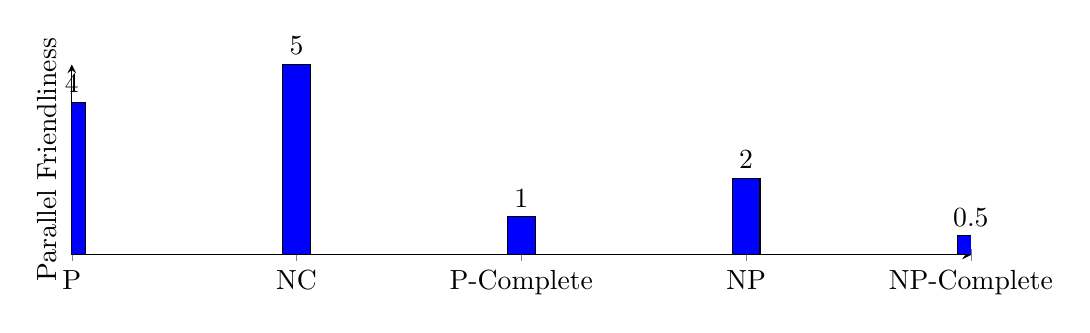
\begin{tikzpicture}
\begin{axis}[
    symbolic x coords={P, NC, P-Complete, NP, NP-Complete},
    xtick=data,
    ymin=0, ymax=5,
    ytick=\empty,
    axis lines=left,
    width=13cm,
    height=4cm,
    nodes near coords,
    every node near coord/.append style={anchor=south},
    ylabel={Parallel Friendliness}
]
\addplot[ybar, fill=blue] coordinates {
    (NC, 5)
    (P, 4)
    (P-Complete, 1)
    (NP, 2)
    (NP-Complete, 0.5)
};
\end{axis}
\end{tikzpicture}
\end{center}

\subsubsection{Conclusion: Parallelism Helps, But Not Always}

Parallelism doesn’t change the nature of a problem—it just distributes the pain. Like integration, its usefulness depends on the \textbf{structure} of the task.

\begin{itemize}
  \item If tasks are independent: parallelism is a silver bullet.
  \item If tasks are chained: parallelism is a band-aid.
  \item If tasks are chaotic: parallelism might make things worse.
\end{itemize}

\begin{quote}
You can’t parallelize causality. You can’t pipeline recursion.  
And you can’t multithread your way out of a gravitational n-body simulation.
\end{quote}



\subsection{Machine Learning and the Brute Force vs. Insight Dilemma}

The challenge of integration in orbital mechanics isn’t just a physics problem—it’s a parable for modern machine learning.

This dilemma isn’t new. John Nash, in his work on game theory, revolutionized our understanding of strategic decision-making by demonstrating that even the most complex problems, like finding an optimal strategy in a competitive environment, could often be tackled not by brute force, but through insight into the structure of the problem. Nash's insight into complexity—particularly his speculation that certain problems would require exponential time to solve—directly parallels the challenge we face today in machine learning and optimization. In a sense, Nash was already hinting at the computational challenges that underlie the problems we tackle in deep learning.

At the heart of every deep learning pipeline lies a brutal question:

\begin{quote} Should we throw compute at it? Or should we think harder and code smarter? \end{quote}

Just like simulating chaotic planetary motion, training large neural networks is an integration problem in disguise. You’re not solving a differential equation, but you are traversing a massive, high-dimensional loss landscape. And as with gravity, the path forward is either:

\begin{itemize} 
	\item Compute-heavy: brute-force optimization with billions of parameters and GPU hours, or 
	\item Insight-driven: clever initialization, architecture tuning, and theoretical grounding. 
\end{itemize}

In fact, Nash’s work in game theory can be seen as an early exploration of this very tradeoff. The "brute-force" approach in game theory would involve exhaustively calculating every possible outcome of a decision-making process. But Nash’s genius lay in realizing that by understanding the underlying structure of these games—by looking for symmetries and equilibrium points—we could find more efficient solutions without having to compute every possibility.

This tradeoff isn’t just academic. It played out in real time with the DeepSeek team.

\subsubsection{Case Study: DeepSeek’s Pivot and the Hidden Cost of Compute}

Originally, the parent company behind DeepSeek wasn’t even an AI lab—it was a high-frequency trading firm that lost its funding. Faced with extinction, they pulled a bold move: pivot to LLMs to show they had machine learning chops.

They didn’t care about chatbots. They wanted investment. Releasing DeepSeek as open source wasn’t about ideology—it was a marketing stunt to save the parent company.

But here’s the twist: it worked.

Because unlike Big Tech, they didn’t have infinite compute. They couldn’t afford to throw teraflops at the wall and wait for a transformer to emerge. So they did something radical: they read the literature.

Everything DeepSeek implemented was already known in academic papers—optimization tricks, scaling laws, model tweaks. Nothing was groundbreaking. But what made it effective was that they actually tried it. They treated machine learning like science, not magic.

Contrast this with the Big Tech approach:

\begin{itemize}
  \item Hire the best engineers in the world.
  \item Throw compute at the problem until it yields.
  \item Accept inefficiency as the price of moving fast.
\end{itemize}

This strategy works—if you have the budget. But not every company does. And not every problem deserves a brute-force solution.

Just like in orbital mechanics, sometimes insight is cheaper than iteration. Sometimes you don’t need more GPUs—you just need a better coordinate system.

\begin{quote}
Deep learning, like gravity, rewards cleverness. But it also punishes laziness with compute bills the size of small nations.
\end{quote}

\textbf{The lesson:} what works for DeepSeek won’t work for Google. And what works for Google might bankrupt a startup. Every company faces the same fundamental choice:

\begin{center}
\textbf{Spend time understanding the problem, or spend money avoiding it.}
\end{center}

There is no one-size-fits-all answer. But there is a rule of thumb: when in doubt, think before you spend. You might just algebrize your way to a breakthrough.


\begin{figure}[H]
  \centering

  % === First row ===
  \begin{subfigure}[t]{0.45\textwidth}
  \centering
  \begin{tikzpicture}
    \comicpanel{0}{0}
      {DeepSeek CEO}
      {}
      {\footnotesize We lost our funding. No more capital, no more leverage, no more free snacks.}
      {(0,-0.6)}
  \end{tikzpicture}
  \caption*{The snack shelves goes dry before the balance sheet does.}
  \end{subfigure}
  \hfill
  \begin{subfigure}[t]{0.45\textwidth}
  \centering
  \begin{tikzpicture}
    \comicpanel{0}{0}
      {DeepSeek COO}
      {}
      {\footnotesize Pivot idea: slap a transformer on it. Maybe investors will bite.}
      {(0,-0.6)}
  \end{tikzpicture}
  \caption*{The “LLM-as-lifeboat” strategy.}
  \end{subfigure}

  \vspace{1em}

  % === Second row ===
  \begin{subfigure}[t]{0.45\textwidth}
  \centering
  \begin{tikzpicture}
    \comicpanel{0}{0}
      {DeepSeek Intern}
      {}
      {\footnotesize We don’t have compute. So we… read the papers?}
      {(0,-0.6)}
  \end{tikzpicture}
  \caption*{No one funds oringial research, but they'll fund a demo with buzzwords.}
  \end{subfigure}
  \hfill
  \begin{subfigure}[t]{0.45\textwidth}
  \centering
  \begin{tikzpicture}
    \comicpanel{0}{0}
      {CCP Official}
      {}
      {\footnotesize They open-sourced it? Yes, that was Step 7 of the 5 year plan... after the Series B manipulation.}
      {(0,-0.6)}
  \end{tikzpicture}
  \caption*{The art of governance: spotting success and claiming it was your idea.}
  \end{subfigure}

  \caption{DeepSeek didn’t innovate—they implemented. A trading firm pivoted to LLMs, ran on desperation and PDFs, and accidentally optimized a geopolitical tool.}
\end{figure}

